\section{Experiment and Analysis}
\label{sec:experimentdesign}
To evaluate the spectrum utility from in-field measurements, we perform experiments 
with an off-the-shelf wireless platform and mobile spectrum analyzer.
%We collect measurements in typical populated areas and sparse areas of DFW metropolitan carrying these platforms. 
According to the measured data, we apply our MAPE framework to analyze the role
of white space and WiFi bands in total access points required for a given deployment area.

\subsection{Experiment Design}
% Platform
%To ensure the results are applicable, 
We employ a Linux-based 802.11 testbed, which includes a Gateworks 2358 board with 
Ubiquiti XR radios (XR9 at 900 MHz, XR2 at 2.4 GHz, XR5 at 5.2 GHz) and a DoodleLabs DL475 
radio at 450 MHz.  We develop shell scripts which utilize tcpdump to enable this testbed to
work as a sniffer, recording all 802.11 packets. However, since the Gateworks platform only 
updates its estimate of received signal strength upon the reception of a new packet (and
not all relevant channel activity is 802.11 based), we employ a a spectrum analyzer to form 
a notion of inter-network interference with finer granularity.  We have Rohde \& Schwarz FSH8 
portable spectrum works from 100 KHz to 8 GHz. The portable spectrum analyzer is controlled 
by a Python script on a laptop measure the received signal strength.

%We perform experiments in downtown Dallas, SMU campus, and neighborhood. The results show
%no 802.11 packets detected in white space bands(450 MHz, 900 MHz) there. 
%And in DFW area, as far as we know, we are the only group holds FCC license of white space bands. 
%Our experiments verify that these bands have not been used for commercial wireless data communication.
%Moreover, we observed that Gateworks platform only update its received signal strength when received
%a new packet.
%It is not good for inter-network interference measurement. To cover the gap,
%we employ a spectrum analyzer, multiband antenna, mobile antenna and a laptop developing
%a spectrum sensing system.

% Data normalize 
To the best of our knowledge, there is no readily availble mobile, multiband antenna from
450 MHz to 5.2 GHz on the market. Thus, we use a 700 MHz mobile antenna to perform in-field
measurements. We then normalize the mobile antenna performance across bands with indoor 
experimentation. To do so, we use a Universal Software Radio Peripheral (USRP) N210 to 
generate signals at 450 MHz, 800 MHz, and 2.4 GHz. We feed the USRP signals directly
to a spectrum analyzer and adjust the configuration of USRP to make the received signal 
strength the same as the 5.2 GHz signal from Gatework 2358 with a XR5 radio. Then, we connect 
the signal source to a fixed multiband antenna (QH 400 Quad Ridge Horn Antenna) and measure the
received signal at a fixed distance with the 700 MHz antenna and antennas for different bands
to get the antenna loss for each band. We adjust the received signal strength
collected via 700 MHz mobile antenna according to the normalization.

  \begin{figure}
  %\vspace{-0.0in}
  \centering
  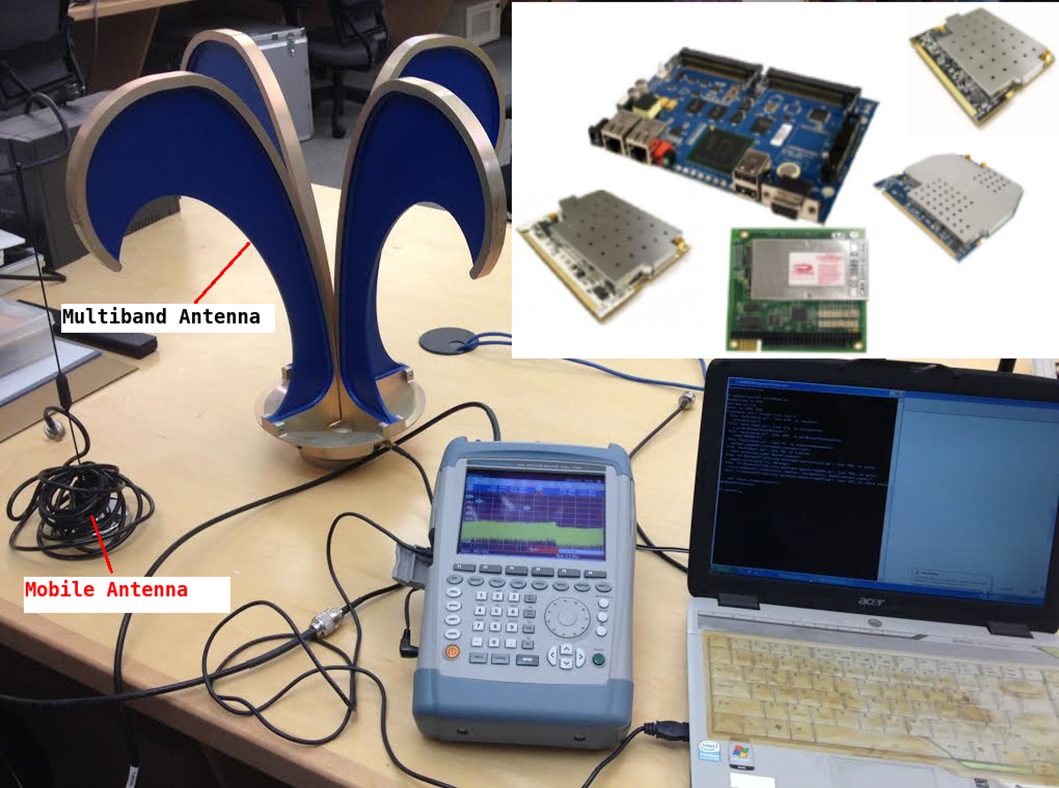
\includegraphics[width=74mm]{figures/equipment}
  \vspace{-0.1in}
  \caption{Multiband Measurement Platform}
  \label{fig:equipment}
  \vspace{-0.2in}
  \end{figure}
  
% Duplicate measurement in WiFi
Our experiment platforms are shown in Figure~\ref{fig:equipment}.
The mobile spectrum analyzer records 32 samples per second on each band under test with 
appropriate time stamps.
The Gateworks sniffer platform also records all the packets received in WiFi bands with time stamps. 
The duplicate samples in WiFi bands from spectrum analyzer and Gateworks are deleted 
according to the time stamp. Then, we calculate the activity level in WiFi bands. 
The activity level of white space bands is calculated based on the spectrum analyzer measurements.  

% Location and Process 
%We apply drive test carrying our platform from Dallas to Weatherford as shown in~\ref{sec:problemformulation}.
%We choose experiments locations according to the population distribution in DFW metropolitan. 
%The experiments are performed in Dallas, Weatherford and Millsap marked with stars in 
%Figure~\ref{fig:drivemap}.
Figure~\ref{fig:drivemap} depicts a map of the available white space channels with
markers where we performed measurements in North Texas. To be representative of a broad range of
community types, we consider populations of approximately 25 times one another according to the
2010 U.S. Census, Millsap (500), Weatherford (25k), and Dallas (1.25 M).
We have collected measurements at multiple types of locations in Dallas, including a downtown area,
a residential area, and a university campus. In Weatherford and Millsap, we monitor wireless activities 
in three locations for 45 minutes on a weekday in downtown, residential, and non-residential areas.
Then, we post-process the data to calculate the activity level of each band in each location.

\subsection{Results and Analysis} 
\label{subsec:result}
In this subsection, we discuss our measurements results and leverage our MAPE framework 
to analyze the influence of white space channels across areas with different population densities.
As an initial experiment, we perform a drive test from Dallas to Weatherford with cruise control 
set to 60 MPH while on the highway. The result of in-field spectrum drive test is shown in 
Figure~\ref{fig:drivetest} according to the location and time of the measurement.
The measured RSSI of 450 MHz is strong in downtown Dallas and Fort Worth 
but has less signal activity in the urban and rural area between these city centers.
The low activity detected in WiFi bands is due to the distance from highway is typically
larger than the propagation range of predominantly indoor wireless routers.
%The map depicted in Figure~\ref{fig:drivemap} shows the available white space channels in DFW area, more green means
%more channels. 
Our initial in-field measurement matches the FCC restrictions (shown in Figure~\ref{fig:drivemap}) with
less channels available translating to greater spectrum utilization.
The drive test also shows that the spectrum utilization seems proportional to the population
density. We use the measurements collected at more fixed locations as marked on the map for
the activity level calculation. 

\begin{figure}
%\vspace{-0.0in}
\centering
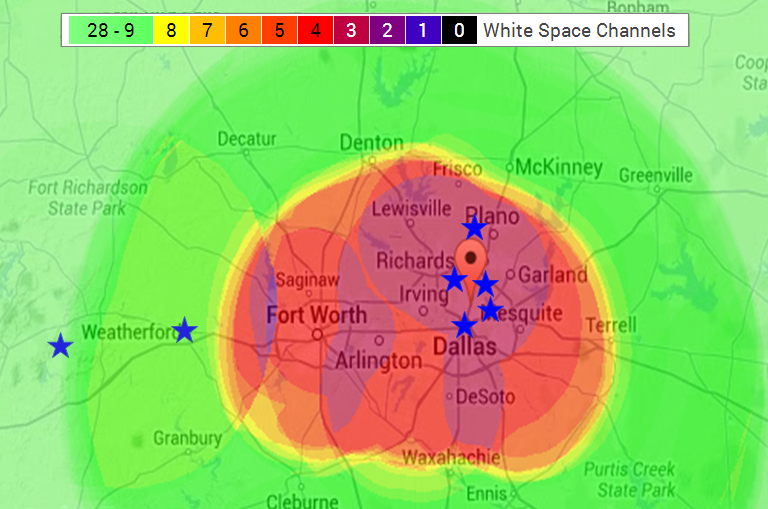
\includegraphics[width=74mm]{figures/drivemap}
\vspace{-0.1in}
\caption{DFW Metropolitan Measurement Location}                                                                 
\label{fig:drivemap}
\vspace{-0.1in}
\end{figure}
   
\begin{figure}
%\vspace{-0.0in}
\centering
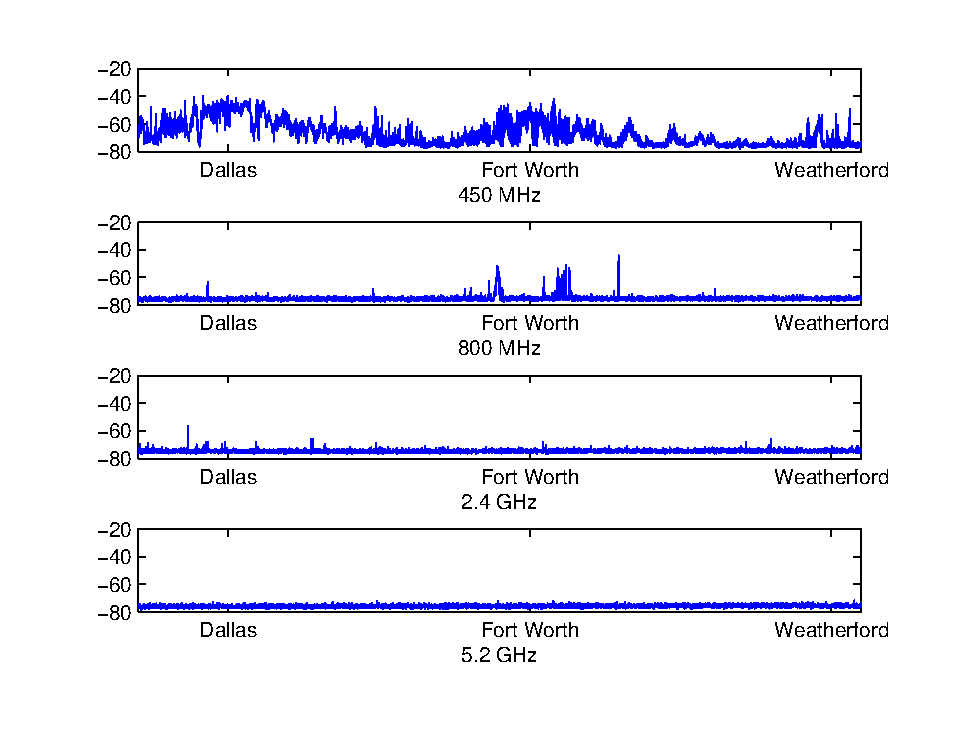
\includegraphics[width=94mm]{figures/drivetest}
\vspace{-0.4in}
\caption{Spectrum Activity In DFW}                                                                 
\label{fig:drivetest}
\vspace{-0.3in}
\end{figure}

The activity level calculated with our measurements are shown in Table~\ref{tab:activitymeasurement}.
Dallas, the city with the greatest population in North Texas, has the highest activity level in most 
of the measured bands, especially at 450 MHz. The measurements of Dallas urban are taken from the SMU 
campus, two neighborhoods, and a densely-populated suburb (Plano). Our meaurements indicate that 2.4 GHz 
has a higher activity level in urban area than the measured downtown area. Most schools and their 
neighborhoods are covered by WiFi, which contributes to the high activity level in 2.4 GHz and 5.2 GHz.
In Weatherford, all the bands have lower activity levels than in Dallas. A peculiarity in the measurements
can be seen by the sparse area in Weatherford having more activity than the other regions for 450 MHz.  
This can be explained due to the measurement location being on the East of Weatherford (closer to Fort Worth,
which has a population of approximately 750k).
Millsap is a typical sparse rural area with approximately 500 total residents. The activity levels across 
all the bands are lower than in Dallas and Weatherford. In the 450 MHz band, the activity level decreases 
much faster than in other bands in Dallas and Weatherford. 

%% Fix location example claiming the activity is kind of stable
%Figure~\ref{fig:labact} depicts an example spectrum utility in activity level
%defined in~\ref{subsec:problem} in our urban lab with the platform introduced 
%in~\ref{sec:experimentdesign}. 
%The activity level from data collected in the same location shows 
%the difference in time domain. On average, the existing signals occupy 25.83 
%percentage of time in 450 MHz, 26.49 percentage of time in 800 MHz, 
%34.95 percentage of time in 2.4 GHz and 35.46 percentage of time in 5.2 GHz. 
%Our experiments show that in a fixed location, the spectrum utility is around
%a certain number in time domain. This character provides a method to tell
%the spectrum utility through measurements. These Inter-network interference 
%of existing signals have to be counted in wireless network deployment. 
%
%   
%In the measurements, there is around $10\%$ difference from white space 
%band to WiFi bands in our urban lab. This spectrum utility gap and multiband
%propagation variation in band selection of wireless network 
%deployment is what we have to notice. 
%
\begin{table*}
\centering % centering table 
\begin{tabular}{|l|c|c|c|c|c|c|c|c|c|c|c|} % creating 12 columns 
\hline %\hline % inserting double-line 
Bands     & \multicolumn{3}{c|}{Dallas} & \multicolumn{3}{c|}{Weatherford} & \multicolumn{3}{c|}{Millsap} \\% [0.5ex]
\hline % inserts single-line 
% Entering 1st row 
Area Type & Downtown & Residential & Suburban & Downtown &  Residential & Sparse & Downtown & Residential & Sparse \\ % [0.5ex]
\hline % inserts single-line 
450 MHz &24.37	&25.83  &23.77	&6.05 &12.50  &14.03 & 7.00 & 0.07 & 0.02 \\      
\hline % inserts single-line                                                                                                       
800 MHz &4.40 	&16.49  &4.77	&5.22&5.07 &4.43  & 3.87 & 4.20 & 3.60 \\      
\hline % inserts single-line                                                                                                      
2.4 GHz &15.87 	&34.95  &2.60	&2.03&2.03 &2.77  & 2.07 & 1.60 & 0.80 \\      
\hline % inserts single-line                                                                                                     
5.2 GHz &19.70	&35.46  &1.53	&1.93&1.93 &1.33  & 1.27 & 2.07 & 2.10 \\      
\hline % inserts single-line 
\end{tabular}    
\label{tab:activitymeasurement}    
\caption{Activity Level in Multiple Locations} % title name of the table 
\vspace{-0.3in}
\end{table*}    

We use the measurement-based activity levels shown in Table~\ref{tab:activitymeasurement} in our framework presented 
in Algorithm~\ref{algorithm:mape}. We specifically use the Millsap sparse area, Millsap downtown, Weatherford residential, Dallas residential, and Dallas 
downtown measurements as inputs of activity level for a given population density.
We then calculate the number of access point for covering 
a 13 km $\times$ 13 km area varying population density. The output is shown in Figure~\ref{fig:redensity}. 

   \begin{figure}
   %\vspace{-0.0in}
   \centering
   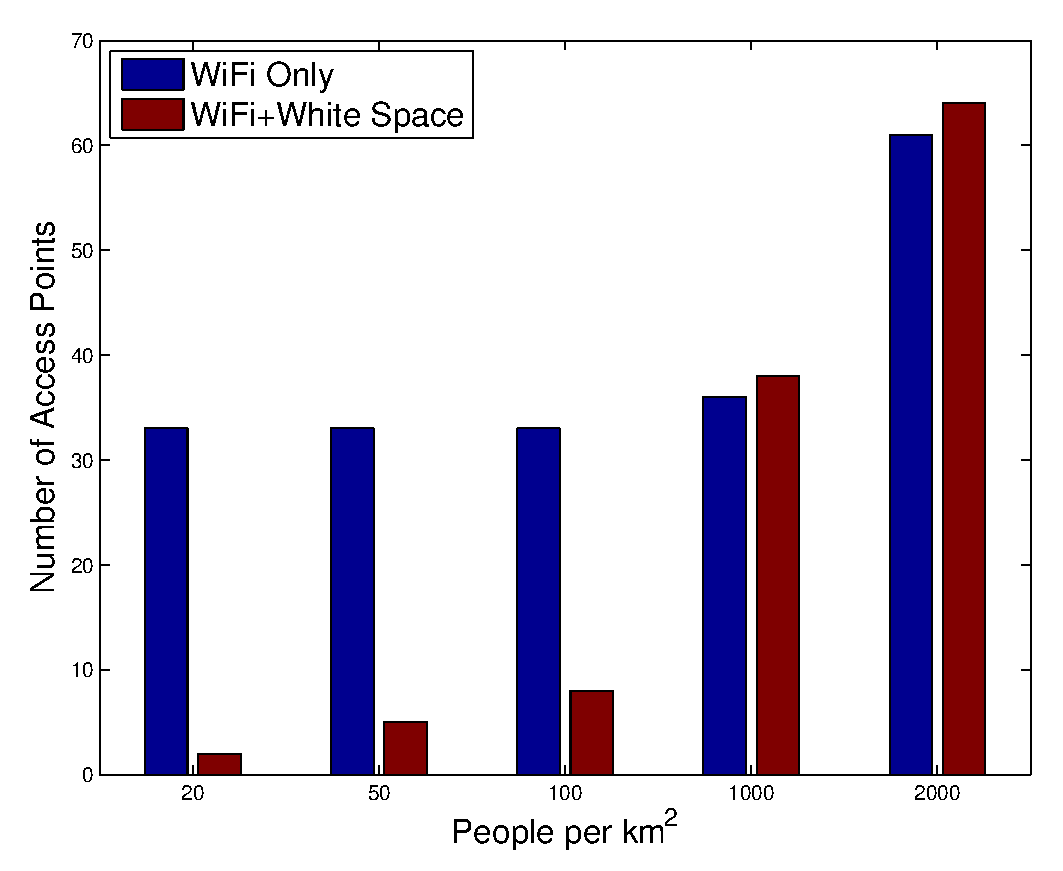
\includegraphics[width=74mm]{figures/redensity}
   \vspace{-0.1in}
   \caption{Number of Access Points need for 13x13 $km^2$ Area}
   \label{fig:redensity}
   \vspace{-0.3in}
   \end{figure}

% Experiment Results & expect results
In the calculation, we set the demand request as 2 Mbps per person with the population
density of 20, 50, 100, 1000, and 2000 per square kilometer. We assume $30\%$ residents will use this
service, the maximum transmit power is 30 dBm, and a path loss exponent of $3.5$~\cite{meikle2012global}. 
For the WiFi Only scenario, we use 6 channels in 2.4 GHz, and 3 channels in 5.2 GHz. 
%Our experiment platforms are shown in Figure~\ref{fig:equipment}.
We adopt an 802.11n maximum data rate of 600 Mbps. For the WiFi+White Space
scenario, we use 3 channels in 450 MHz, 2.4 GHz and 5.2 GHz each. Each of these scenarios have the 
same channels in total (9). As shown in Figure~\ref{fig:redensity},
with the same number of channels, WiFi+White Space reduces the number of access points by $1650\%$ compared to WiFi Only in the
20 people per square km scenario, $660\%$ in the 50 people per square km, and $412.5\%$ in the 100 people
per square km scenario. However, as the population density increases, due to the capacity constraint of servicing
people in this area, the lower frequency white space bands lose their advantage of larger communication range. 
At the same time, the activities of other signal sources, such as TV stations in downtown areas, reduce
the capacity of white space bands. As a result, the WiFi+White Space scenario performs worse than the WiFi Only scenario.
If we were to count the intra-network interference (out of scope), the situation could become even worse.
Moreover, FCC has stricter policies on white spaces in urban area. Fewer channels
are available in these areas, which makes WiFi a better option for dense areas.

To understand the influence of band combinations on network deployments, we calculate the number of 
access points in the area when selecting 500 people per square km with a downtown Weatherford spectrum 
utilization and 1500 people per square km with a residential Dallas spectrum utilization.
We assume the total number of channels is 12. We use the same setup 
as the previous experiment. %The results are shown in Figure~\ref{tab:500comb}.
 
 \begin{table}[h]
 \centering
 \begin{tabular}{|c|c|c|c|}
 \hline
 \multirow{2}{*}{No. of Bands} & \multirow{2}{*}{Bands Combination} & \multicolumn{2}{c|}{No. of AP} \\
 \cline{3-4}
  &  & 500 & 1500 \\
 & (Hz) & $ppl/km^2$ &  $ppl/km^2$ \\
 \hline
 \multirow{4}{*}{1}    & 450 M  & 12  & 35 \\
 \cline{2-4}
                              & 800 M & 10  &  30 \\
 \cline{2-4}
			      & 2.4 GHz & 33  &  37 \\
 \cline{2-4}
                              & 5.2 G & 193 &  193 \\ 
 \hline
 \multirow{6}{*}{2}   & 450 M,800 M & 11  & 32\\
 \cline{2-4}
                              & 450 M,2.4 G & 23  & 36\\
 \cline{2-4}
			      & 450 M,5.2 G & 23  & 69\\
 \cline{2-4}
			      & 800 M,2.4 G & 20  & 33\\ 
 \cline{2-4}
			      & 800 M,5.2 G & 20  & 59\\ 
 \cline{2-4}
			      & 2.4 G,5.2 G & 33  & 73\\ 
 \hline
 \multirow{4}{*}{3} & 450 M,800 M,2.4 G & 16  & 33\\
 \cline{2-4}
                              & 450 M,800 M,5.2 G & 16  & 48\\
 \cline{2-4}
			      & 450 M,2.4 G,5.2 G & 33  & 53\\
 \cline{2-4}
			      & 800 M,2.4 G,5.2 G & 30 &  49\\ 
 \hline
 4  & 450 M,800 M,2.4 G,5.2 G & 21  & 44 \\
 \hline
 \end{tabular}
 \caption{Channel Combinations for $500$ and $1500$ Population Density Scenarios}
 \label{tab:500comb}
 \vspace{-0.2in}
 \end{table}


In Table~\ref{tab:500comb}, we compare the number of access points with 12 channels through all 
the possible combinations of bands. 
% Single band compare
When all the channels are in the same band, as the frequency goes up, more access 
points are needed to serve the area due to the limited propagation range. However,
450 MHz does not outperform 800 MHz with a single band at both the 500 and 1500 people per
square km cases because 450 MHz channels have larger measured activity levels. 
White space band channels outperform WiFi bands by up to 1830\% in single band case
with 500 people per square km case, but with 1,500 people per square km, the cost reduction
decreases to only 543\%.
% Two bands 
We now distribute an equal number of channels to two-band combinations and run the experiments 
with the same population densities and spectrum utilization. The results shows the white space band
combination (450 and 800 MHz) performs better than WiFi only (2.4 and 5.2 GHz) by 200\% and
128\% with the people per square km of 500 and 1,500, respectively. In fact, the only white space 
scenario (450 and 800 MHz) has almost the same performance as the scenarios with one white band and
one WiFi band (450 MHz and 2.4 GHz; 800 MHz and 2.4 GHz) with 1,500 people per square km.
However, with 500 people per square km, the white space only is much better than any other two-band combination.
% Three bands
White space channels provide up to 87.5\% cost reduction in three-band combination scenarios with
500 people per square km nad up to 33.3\% with 1,500 people per square km.  With four bands,
the number of access points required does not reduce using white space bands.

From Figure~\ref{fig:redensity} and Table~\ref{tab:500comb}, we show that as the population
density increases, the reduction in number of access points required to meet the same demand 
diminishes. Note that a more optimal allocation of channels in different bands could offer
further cost reductions. We further show that as population and spectrum utilization increase, 
at some point, the performance of white space only scenario could be the same as a combination of
white space and WiFi bands. 
%Then we may pay
%less money to get less number of white space channels for wireless net work deployment.

